\documentclass[12pt]{article}
\usepackage[margin=1in]{geometry}
\usepackage[pdftex]{graphicx}
\usepackage{amsmath,amssymb,amsthm}
\usepackage{float}
\usepackage{custom}
\usepackage{pgfplots}
\usepackage{tikz}
\usepackage{tasks}
% \usepackage{times}
\usepackage{lmodern}

% color boxes
\usepackage[many]{tcolorbox}
\tcbuselibrary{theorems}
\newtcbtheorem{pssolution}{Solution}{colback=orange!10,colframe=orange!40!black,fonttitle=\bfseries,breakable,enhanced}{sn}
\tcbset{noparskip/.style={before={\par\pagebreak[0]\medskip\parindent=0pt},
after={\par\medskip}}}

% code for totaling up points 
\usepackage{totcount}
\newtotcounter{tpts}
\newtotcounter{cpts}
\newtotcounter{endpts}
\newcommand{\clearpts}{\addtocounter{tpts}{\value{cpts}} \setcounter{cpts}{0}}
\newcommand{\pts}[1]{\clearpts \setcounter{cpts}{#1}}
\newcommand{\totpts}{\setcounter{endpts}{\totvalue{tpts} + \totvalue{cpts}}\arabic{endpts}}

% formatting for problems and solutions
\definecolor{ptred}{rgb}{0.7,0.1,0.1}
\newcommand{\ptfmt}[1]{\textbf{\color{ptred}#1\color{black}}}
\definecolor{advblue}{rgb}{0.1,0.1,0.7}
\newcommand{\advanced}{\!\textbf{\color{advblue}[A]\color{black}}\ }

\newtheorem*{solution}{Solution}
\newtheorem*{answer}{Answer}

\makeatletter
\newtheoremstyle{mystyle}
{\topsep}               % space above
{\topsep}               % space below
{}                      % bodyfont
{}                      % indent
{\bfseries}             % headfont
{}                      % punctuation
{0.6em}                 % space after head
{\llap{[\ptfmt{\arabic{cpts}}]\hspace{.6em}}\thmname{#1}\thmnumber{ #2}\thmnote{\normalfont{ (#3)}}{\bfseries .}}  %theoremheadspec
\theoremstyle{mystyle}
\newtheorem{pproblem}{Problem}
\makeatother

% ------------- MOCK TITLE ------------- %
\newcommand\mocktitle{Rotations}
% -------------------------------------- %


% headers and footers
\usepackage{fancyhdr}
\pagestyle{fancy}
\lhead{\href{https://activities.tjhsst.edu/physics/index.html}{TJHSST Physics Team}}
\rhead{\thepage}
\cfoot{\href{https://activities.tjhsst.edu/physics/index.html}{TJHSST Physics Team}}
\renewcommand{\headrulewidth}{0.4pt}
\setlength{\headheight}{15pt}

\newcommand{\psettitle}[1]{
    \begin{center}
    \huge \textbf{#1}
    \end{center}
}

\linespread{1.03} % give a little extra room
\setlength{\parindent}{0.2in} % reduce paragraph indent a bit

% uncomment to hide solutions
%\usepackage{environ}
%\NewEnviron{hide}{}
%\let\solution\hide
%\let\endsolution\endhide
%\let\answer\hide
%\let\endanswer\endhide

% tikz setup
\usetikzlibrary{calc, decorations.pathreplacing, decorations.pathmorphing, angles, quotes, positioning, patterns}
\tikzstyle{arrow} = [thick,->,>=stealth]
\newcommand{\AxisRotater}[1][rotate=0]{
  \tikz [x=0.25cm,y=0.60cm,line width=.2ex,-stealth,#1] \draw (0,0) arc (-150:150:1 and 1);
}

\pgfplotsset{compat=1.18}

\begin{document}

\begin{center}
    \Large \textbf{\mocktitle\ Mock Exam} \vspace{4mm}
    
    \Large 10 MCQ 2 FRQ - 60 MINUTES \vspace{4mm}
    
    \Large \textbf{INSTRUCTIONS} \linebreak[2]
    
    \normalsize \textbf{DO NOT OPEN THIS TEST UNTIL YOU ARE TOLD TO BEGIN}
\end{center}

\begin{itemize}
    \item Use $g = 9.8$ N/kg throughout this contest.
    \item Test under standard conditions, which means that you must complete the test in 60 minutes in one sitting.
    \item This test contains 10 Multiple Choice Questions and 2 Free Response Questions.
    \item Correct answers will be awarded the points shown; leaving an answer blank will be awarded zero points. The amount of partial credit is up to your discretion as the grader. Our recommendation is to be more strict than necessary.
    \item A hand-held calculator may be used. Its memory must be cleared of data and programs. You may use only the basic functions found on a graphing calculator. Calculators may not be shared. Cell phones may not be used during the exam. You may not use tables, books, or formula collections.
    \item The number in \ptfmt{red} next to each question represents the amount of points the question is worth. There are a total of 40 points on this test.
    \item If you have any questions or clarifications, please contact us at \href{mailto:tjhsstphysicsteam@gmail.com}{tjhsstphysicsteam@gmail.com}.
\end{itemize}
\vspace{7mm}

The creators of this exam are (in alphabetical order):
\vspace{1mm}
% Please add your name in alphabetical order
\begin{center}
    \textit{Aarush Deshpande, Eric Xie}
\end{center}

Good luck and have fun! Turn the page to start the mock.

\newpage

\subsection*{10 MCQs}
\pts{2}
\begin{pproblem}
    A wheel of radius $R$ is rolling without slipping with an angular velocity
    $\omega$. For a point $A$ on the wheel at an angle $\theta$ with respect
    to the vertical, what is the magnitude of the velocity with respect
    to the ground?

    \begin{figure}[H]
        \centering
        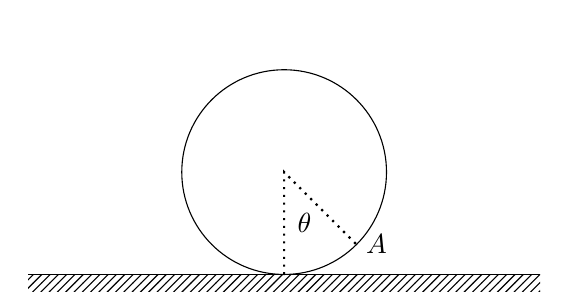
\begin{tikzpicture}[scale=1.3]
            \draw (0,0) -- (5,0);
            \fill [pattern = north east lines] (0,0) rectangle (5,-.3);
            \draw (2.5, 1) circle (1);
            \draw[dotted,thick] (2.5, 0) -- (2.5, 1) -- (3.2,0.3) node[right] {$A$};
            \node at (2.7,0.5) {$\theta$};
        \end{tikzpicture}
    \end{figure}
    \begin{enumerate}[label=(\Alph*)]
        \item $\omega R$
        \item $\omega R\sin(\left|\theta\right|/2)$
        \item $\sqrt{2}\omega R\sin(\left|\theta\right|/2)$
        \item $2\omega R\sin(\left|\theta\right|)$
        \item $2\omega R\sin(\left|\theta\right|/2)$
    \end{enumerate}
\end{pproblem}
\begin{solution}
    The velocity has a contribution from the movement of the center of mass, and 
    from the rotation itself: \[
        \mathbf{v}=\mathbf{v}_\mathrm{CM}+\mathbf{v}_\mathrm{tangential}
    \]
    Because it's rolling without slipping, we have
    $v_\mathrm{CM}=\omega R$. The tangential velocity is $\omega R$ as well.
    
    Splitting the tangential velocity into components, we have
    \begin{align*}
        \left\vert\mathbf{v}\right\vert &= \sqrt{(\omega R\sin\theta)^2+(\omega R-\omega R\cos\theta)}\\
        &=\sqrt{2}\omega R\sqrt{1-\cos\theta}\\
        &=2\omega R\sin\left\vert\dfrac{\theta}{2}\right\vert
    \end{align*}
    or \fbox{E}.
\end{solution}

% Maybe too hard?
\pts{2}
\begin{pproblem}
    A spring with a spring constant $k_1$ is attached to another spring with a spring constant
    $k_2$. $k_2$ is then attached to a mass, and the system begins to oscillate.
    The period of oscillation of the system
    is of the form, \[
        T=2\pi\sqrt{\dfrac{m}{k_\mathrm{eff}}}
    \]
    What is $k_\mathrm{eff}$?
    \begin{figure}[H]
        \centering
        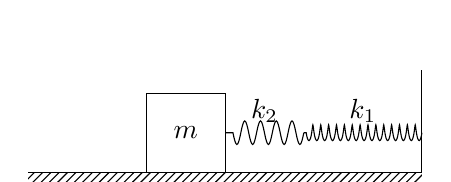
\begin{tikzpicture}
            \draw (0,0) -- (5,0);
            \fill [pattern = north east lines] (0,0) rectangle (5,-.3);
            \draw (5,0) -- (5,1.3);
            \draw [decoration={aspect=0.1, segment length=1mm, amplitude=1mm,coil},decorate]
                (5,.5) -- (3.5,.5) node[midway, above] {$k_1$};
            \draw [decoration={aspect=0, segment length=2mm, amplitude=1.5mm,coil},decorate]
                (3.5,.5) -- (2.5,.5) node[midway, above] {$k_2$};
            \draw (1.5,1) rectangle (2.5,0) node[midway] {$m$};
        \end{tikzpicture}
    \end{figure}
    \begin{enumerate}[label=(\Alph*)]
        \item $k_\mathrm{eff}=\dfrac{k_1k_2}{k_1+k_2}$
        \item $k_\mathrm{eff}=\dfrac{k_1+k_2}{2}$
        \item $k_\mathrm{eff}=k_1+k_2$
        \item $k_\mathrm{eff}=\left(\dfrac{k_1}{k_2}\right)(k_1-k_2)$
        \item $k_\mathrm{eff}=\left(\dfrac{k_1}{k_2}\right)(k_1+k_2)$
    \end{enumerate}
\end{pproblem}
\begin{solution}
    Note that if we only had a spring with spring constant $k_1$, $k_\mathrm{eff}=k_1$.
    As such, the question is asking us to simplify this problem to effectively
    having only one spring. Therefore, the force on the mass must be
    $F_\mathrm{net}=-k_\mathrm{eff}(x_1+x_2)$,
    where $x_1$ and $x_2$ are the changes in length of spring 1 and 2, respectively.

    Force balancing at the intersection of the two springs gives \[
        k_2x_2=k_1x_1\implies x_1=\dfrac{k_2}{k_1}x_2
    \]
    Substituting the following gives \[
        F_\mathrm{net}=-k_\mathrm{eff}x_2\left(1+\dfrac{k_2}{k_1}\right)
    \]
    Now, by force balance on the mass, we have the only force acting on it to be spring 2.
    Therefore, $F_\mathrm{net}=-k_2x_2$. Setting the two equations equal gives us \[
        k_\mathrm{eff}=\dfrac{k_1k_2}{k_1+k_2}
    \] or \fbox{A}.

    This arrangement of springs is called being in \textit{series}.
\end{solution}


\pts{2}
\begin{pproblem}
    Two \textit{rings} of radius $R=2$ m and mass $1$ kg are attached a distance $R$ apart, as shown in Figure \ref{two-circles}. They rotate about a point $A$ at the intersection
    of the two circles, with an angular velocity $4$ rad/s.
    What is the angular momentum of the system, about an axis perpendicular to the
    paper and going through the point $A$?

    \begin{figure}[H]
        \centering
        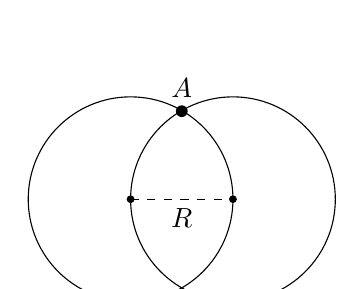
\begin{tikzpicture}[scale=1.3]
            \draw (-.5,0) circle (1);
            \node at (-.5,0)[circle,fill,inner sep=1pt]{};
            \draw (.5,0) circle (1);
            \node at (.5,0)[circle,fill,inner sep=1pt]{};
            \node at (0,.86)[circle,fill,inner sep=1.5pt]{};
            \node at (0,0.9)[above]{$A$};
            \draw[dashed] (-.5,0) -- (.5,0) node[midway,below] {$R$};
        \end{tikzpicture}
        \label{two-circles}
    \end{figure}
    \begin{enumerate}[(\Alph*)]
        \item $16\mathrm{kg\cdot m^2/s}$
        \item $32\mathrm{kg\cdot m^2/s}$
        \item $48\mathrm{kg\cdot m^2/s}$
        \item $64\mathrm{kg\cdot m^2/s}$
        \item $76\mathrm{kg\cdot m^2/s}$
    \end{enumerate}
\end{pproblem}
\begin{solution}
    The moment of inertia of a ring about it's center of mass is $mR^2$, so by
    the parallel axis theorem the moment of inertia about one of its radii is \[
        I_r=mR^2+mR^2=2mR^2
    \]
    Therefore the angular momentum of one ring is $I_r\omega$. However, we have two
    rings, so the angular momentum of the system is $2I_r\omega=4mR^2\omega=64\mathrm{kg\cdot m^2/s}$, or \fbox{D}.
\end{solution}

% -------------------------------- %
%             Too Bashy?           %
% -------------------------------- %
\pts{2}
\begin{pproblem}
    Aarush holds a stick of mass $m$ and length $\ell$ on one end, hanging down.
    Eric shoots a ball of mass $m$ with velocity $v$, and it collides inelastically with
    the stick a distance $x=d$ from the top. What is the value of $d$ for which Aarush
    doesn't feel a sting from the collision? Alternatively, at what value of $d$ does
    the edge of the stick not move at the instant of collision if Aarush had not held the end in place? Ignore any effects from gravity.
    
    The moment of inertia of a stick of length $\ell$ about an axis perpendicular to the
    plane going through its center of mass is $m\ell^2/12$.

    \begin{figure}[H]
        \centering
        \begin{tikzpicture}
            \draw[thick] (0,0) -- (0,5) node[circle, fill,inner sep=1.5pt]{};
            \node[circle,fill,inner sep=1.5pt] (ball) at (-2,1) {};
            \node[below] at (ball) {$m$};
            \draw[-stealth,thick] (ball) -- +(1,0) node[midway, above] {$v$};
            % brace
            \draw[decorate,decoration={brace,amplitude=10pt,raise=1ex}] (0,5) -- (0,1)
                node[midway, right, xshift=15pt] {$d$};
        \end{tikzpicture}
    \end{figure}
    \begin{enumerate}[(\Alph*)]
        \item $\dfrac{\ell}{3}$
        \item $\dfrac{\ell}{2}$
        \item $\dfrac{2\ell}{3}$
        \item $\dfrac{3\ell}{4}$
        \item $\dfrac{5\ell}{6}$
    \end{enumerate}
\end{pproblem}
\begin{solution}
    If Aarush does not initially feel the impact of the collision, then the top end of the rod remains stationary (like a pivot) even though Aarush does not exert a force on the rod. Since there are no external forces or external torques on the rod-ball system, we may use conservation of linear momentum and conservation of angular momentum. 
    Starting with angular momentum conservation, the initial angular momentum of the ball is:
    $$L_i = mvd$$
    The rod is initially stationary, so this is the total initial angular momentum of the system. Following the collision, the ball sticks to the rod, so we let the contact point move with velocity $v'$. The total angular momentum can be found by adding up the angular momenta of the ball and the rod:
    $$L_{\text{ball}} = mv'd$$
    $$L_{\text{rod}} = I\omega = \frac{1}{3}ml^2\omega$$
    Since the contact point is a distance d from the pivot, $\omega = \frac
    {v'}{d}$. Therefore,
    $$L_{\text{rod}} = I\omega = \frac{ml^2v'}{3d}$$
    Solving for v', 
    $$L_i = L_f = L_{\text{ball}} + L_{\text{rod}}$$
    $$mvd = mv'd + \frac{ml^2}{3d}v'$$

    Using conservation of linear momentum, 
    $$mv = mv' + mv_{\text{cm}}$$
    Since $v_{\text{cm}} = \omega \frac{l}{2} = \frac{lv'}{2d}$
    $$mv = mv' + \frac{mlv'}{2d}$$
    Multiplying by d, 
    $$mvd = mv'd + \frac{mlv'}{2}$$
    Combining this with our equation for conservation of angular momentum:
    $$mv'd + \frac{mlv'}{2} = mv'd + \frac{ml^2}{3d}v'$$
    Therefore, $d = \frac{2l}{3}$, or \boxed{C}
\end{solution}

\pts{2}
\begin{pproblem}
    The following shapes roll without slipping down an inclined plane of angle $\theta$,
    and length $\ell$:
    \begin{enumerate}[align=left]
        \item A disk of mass $m$ and radius $R$.
        \item A spherical shell of mass $m$ and radius $R$.
        \item A spherical shell of mass $2m$ and radius $R/2$.
        \item A sphere of mass $m$ and radius $R$
        \item A sphere of mass $2m$ and radius $R$
    \end{enumerate}
    Given the moments of inertia are $2mR^2/3$ for a spherical shell, 
    $2mR^2/5$ for a solid sphere, and $mR^2/2$ for a disk, rank the times taken for
    each shape to reach the bottom of the inclined plane.

    \begin{enumerate}[label=(\Alph*)]
        \item $T_1 = T_2 = T_3 = T_4 = T_5$
        \item $T_1 < T_2 < T_3 < T_4 < T_5$
        \item $T_1 < T_2 = T_4 < T_3 = T_5$
        \item $T_2 = T_3 < T_1 < T_4 = T_5$
        \item $T_3 < T_2 < T_1 < T_4 < T_5$
        \item $T_3 < T_2 = T_5 < T_1 < T_4$
        \item $T_4 = T_5 < T_1 < T_2 = T_3$
        \item $T_4 < T_1 < T_5 < T_2 = T_3$
        \item $T_5 < T_3 < T_4 < T_1 < T_2$
        \item $T_5 < T_3 < T_1 < T_4 < T_2$
    \end{enumerate}
\end{pproblem}
\begin{solution}
    Let us find the acceleration down the inclined plane for a shape with a moment
    of inertia of the form $\beta mR^2$, where $\beta$ is a constant.

    In such a case, take the axis as the point where the shape and the inclined
    plane meet. In such a base, the moment of inertia is
    $I_\mathrm{new}=\beta mR^2+mR^2=(1+\beta)mR^2$, by the
    parallel axis theorem.
    The torque contributed by friction and the normal force thus have
    a lever arm of 0, and the only force giving a torque is gravity. The torque due
    to gravity is then \[\tau=mgR\sin\theta\]
    Using $\tau=I_\mathrm{new}\alpha$, we then have \[
        mgR\sin\theta=I_\mathrm{new}\alpha=(1+\beta) mR^2\alpha
    \]
    Since the shapes roll without slipping, we have $a=\alpha R$, and so
    $a\propto 1/(1+\beta)$. For a constant distance, we have by the
    kinematic equations that $t\propto a^{-1/2}$ so the ones that roll
    down the fastest have the lowest coefficient for the moment of inertia.
    Note that the acceleration is independent of mass and radius!

    Therefore, we end up with sphere $<$ disk $<$ shell, or \fbox{G}.
\end{solution}

\pts{2}
\begin{pproblem}
    A thin slab of mass $m$ and length $\ell$ hangs over a ledge. There is a pivot on the left end of the slab that allows it to rotate about that point. A bullet of mass $m$ and velocity $v$ hits the bottom-right edge of the slab as shown and gets stuck inside it. The slab eventually comes to rest perfectly vertically. Given that the moment of inertia of a slab
    about its tip is $m\ell^2/3$, find $v$.
    
    \begin{figure}[H]
        \centering
        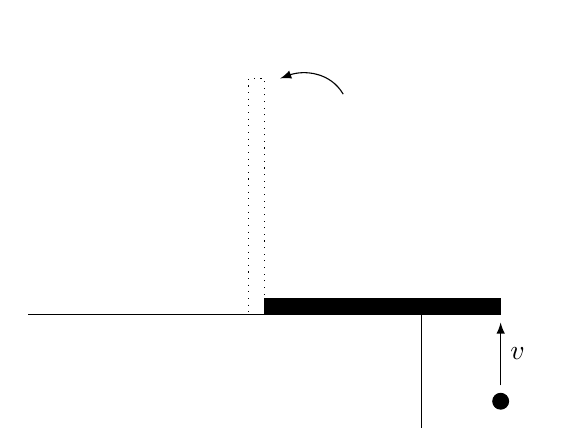
\begin{tikzpicture}
            \draw (-5, 0) -- (0, 0) -- (0, -1.6);
            \draw[fill=black] (-2, .2) rectangle (1, 0);
            \draw[dotted] (-2, 0) rectangle (-2.2, 3);
            \draw[fill=black] (1, -1.1) circle (0.1);
            \draw [-latex] (-1, 2.8) to [out=120,in=20] (-1.8, 3);
            \draw [-latex] (1, -.9) -- (1, -.1) node[midway, right]{$v$};
        \end{tikzpicture}
    \end{figure}
    
    \begin{enumerate}[(\Alph*)]
        \item $2\sqrt{gl}$
        \item $\sqrt{3g\ell}$
        \item $\sqrt{2g\ell}$
        \item $\sqrt{g\ell}$
        \item $\sqrt{\dfrac{8g\ell}{3}}$
    \end{enumerate}
\end{pproblem}
\begin{solution}
    First, note that we will have to use conservation of angular momentum to find the
    angular velocity after the collision, followed by
    conservation of energy to get the result. Conservation of linear momentum does
    not work, because the table exerts a non-negligible normal force (due to the
    slab being rigid). Also, just using conservation of energy does not work because
    energy is lost in the inelastic collision.

    Conserving angular momentum gives us
    \begin{align*}
       mv\ell&=\left(\dfrac{1}{3}m\ell^2+m\ell^2\right)\omega\\
       \implies \omega&=\dfrac{mv}{4m\ell^2/3}
    \end{align*}
    When conserving energy, we have to be careful to use $\ell/2$ as the height
    for the slab, because that's the height of it's center of mass.
    \begin{align*}
        \dfrac{1}{2}\left(\dfrac{1}{3}m\ell^2+m\ell^2\right)\omega^2 &= mg\dfrac{\ell}{2}+mgl\\
        \dfrac{3mv^2}{8} &= \dfrac{3}{2}mg\ell\\
        \implies v &= 2\sqrt{gl}
    \end{align*}
    or \fbox{A}.
\end{solution}


\pts{2}
\begin{pproblem}
    A thin disk of mass $M$ and radius $R$ is rotating about its central axis at an
    angular velocity $\omega_0$. The disk has a very small hole made at a distance $R/3$
    from its center. The hole is suddenly covered by a rod, and the rod stays at rest
    afterward. With what angular velocity does the disk start to rotate? Assume the disk
    is lying on a frictionless surface. The moment of inertia of a disk about its center
    is $MR^2/2$.
    \begin{enumerate}[label = (\Alph*)]
        \item $2\omega_0/3$
        \item $5\omega_0/8$
        \item $7\omega_0/13$
        \item $6\omega_0/7$
        \item $9\omega_0/11$
    \end{enumerate}
\end{pproblem}
\begin{solution}
    Following the insertion of the rod, the rod exerts a large force to cause the disk to start rotating about that axis. Because these forces act at the hole, there is no torque about this point. Therefore, angular momentum is conserved about this point.

    Since the center of mass of the disk does not move, the initial angular momentum is $$L_i = I\omega = \frac{1}{2}MR^2\omega_0$$. The final angular momentum is $L_f = I_f\omega_f$, where $I_f$ and $\omega_f$ are the final moments of inertia and angular velocities around the pivot point. 

    Using the parallel axis theorem, the moment of inertia about the rod is:
    $$I_f = I_{\text{cm}} + Md^2$$ where d is the distance between the rod and the center of mass of the disk. Since $d = R/3$ and $I_{\text{cm}} = \frac{1}{2}MR^2$, 
    $$I_f = \frac{1}{2}MR^2 + \frac{1}{9}MR^2 = \frac{11}{18}MR^2$$
    The initial and final angular momenta must be equal to each other, so $\omega = \frac{L_i}{I_f} = \frac{\frac{1}{2}MR^2\omega_0}{\frac{11}{18}MR^2}$. The final angular velocity must then be: $\omega = \frac{9}{11}\omega_0$, or \boxed{E}
\end{solution}

\pts{2}
\begin{pproblem}
    A disk of radius 5 meters starts at rest at time $t = 0$. It undergoes uniform angular acceleration. At time $t = 3$, a point on the rim is now moving at 7.5 m/s. At time $t = 3$, what is the magnitude of the net acceleration that a particle 3 meters from the center experiences, assuming that the disk continues accelerating at time $t = 3$? 
    \begin{enumerate}[label = (\Alph*)]
        \item 1.50 $\mathrm{m/s^2}$ 
        \item 6.75 $\mathrm{m/s^2}$ 
        \item 6.91 $\mathrm{m/s^2}$ 
        \item 8.73 $\mathrm{m/s^2}$ 
        \item 9.02 $\mathrm{m/s^2}$ 
    \end{enumerate}
\end{pproblem}
\begin{solution}
    The net acceleration of the particle consists of two parts: an acceleration in the tangential direction due to the angular acceleration and a centripetal acceleration in the radial in direction. 

    At time t=3, the angular velocity of the disk, using the point on the rim, is given by $\omega = \frac{v}{R} = \frac{7.5}{5} = 1.5$ $s^{-1}$. Since the angular acceleration was constant, $\alpha = \frac{\omega}{t} = \frac{1.5}{3} = 0.5$ $s^{-2}$. The acceleration in the tangential direction is then
    $$a_\theta = \alpha r = 0.5*3 = 1.5\text{ }m/s^{2}$$ where we plugged in $r = 3$ since the particle is a distance of 3 meters from the center of the disk. 

    The centripetal acceleration of the particle is
    $$a_r = \frac{v^2}{r}$$ where again $r = 3$ and the velocity can be found using $v = \omega r = 1.5*3 = 4.5$. Therefore, $a_r = \frac{4.5^2}{3} = 6.75$
    The magnitude of the acceleration would then be $a = \sqrt{a_r^2 + a_\theta^2} = \sqrt{6.75^2 + 1.5^2} = 6.91$, or \boxed{C}
\end{solution}

\pts{2}
\begin{pproblem}
    Figure \ref{skew rod} shows a rotating skew rod. Two objects of mass $3$ kg are attached to a rod a distance $4$m away from the axis of rotation,
    such that the angular momentum L of the system about its center is at an angle $\alpha=20^\circ$ from the vertical, and
    the rod is spinning with an angular speed $\omega=3\mathrm{rad/s}$. Which of the following is the closest to the magnitude of $\mathbf{L}$?

    \begin{figure}[H]
        \centering
        \begin{tikzpicture}
            \coordinate (intersection) at (2,1);
            \coordinate (rodtip) at (2,4);
            \coordinate (vectortip) at (3,2.5);
    
            \draw (-1,3) -- (5,-1);
            \filldraw (-1,3) circle (2pt) node[above] {$3$kg};
            \filldraw (5,-1) circle (2pt) node[above] {$3$kg};
            \draw[line width=0.5mm] (2,-1) -- (rodtip);
            \node at (1.9,3)
              {\AxisRotater[rotate=-90,y=0.4cm]};
            \node at (2.7,3.2) {$\omega$};
            \draw[-stealth] (2,1) -- (vectortip) node[above right]{$\mathbf L$};
            \pic[draw, -, "$\alpha$", angle eccentricity=1.5] {
              angle=vectortip--intersection--rodtip
            };
        \end{tikzpicture}
        \caption{A Rotating Skew Rod}
        \label{skew rod}
    \end{figure}
    \begin{enumerate}[(\Alph*)]
        \item $250\mathrm{\dfrac{kg\cdot m^2}{s}}$
        \item $270\mathrm{\dfrac{kg\cdot m^2}{s}}$
        \item $290\mathrm{\dfrac{kg\cdot m^2}{s}}$
        \item $310\mathrm{\dfrac{kg\cdot m^2}{s}}$
        \item $330\mathrm{\dfrac{kg\cdot m^2}{s}}$
    \end{enumerate}
\end{pproblem}
\begin{solution}
    The angular velocities for both objects point up, so the structure must rotate counterclockwise (as seen from above). The left object has a velocity pointing out of the page, while the right object has a velocity pointing into the page. Using the formula for angular momentum $\Vec{L} = \Vec{r} \times m\Vec{v}$, the angular momenta of both objects point in the direction of $\Vec{L}$ shown in the figure. The magnitude of each object's angular momentum is $mvl$, where l is the distance from the center of the rod to either object. 
    
    The velocity of the masses can be found using $$v = \omega r$$ where r is the perpendicular distance from the axis of rotation to either particle and is clearly $l\cos \alpha$. Therefore, the total angular momentum of the system is 
    $$2ml^2\omega \cos \alpha$$
    Plugging in all values, we find the angular momentum to be $270\mathrm{\dfrac{kg\cdot m^2}{s}}$, or \boxed{B}
\end{solution}


\begin{pproblem}
    One end of a stick of mass $m$ and length $\ell$ is pivoted against a wall,
    and the other end rests on a frictionless floor (see Figure \ref{pivoted plane}).
    Let $F_l$ and $F_R$ be the vertical forces on the left and right ends of the stick,
    respectively. Then:
    \begin{enumerate}[(\Alph*)]
        \item $F_L>F_R$
        \item $F_L<F_R$
        \item $F_L=F_R=mg/2$
        \item $F_L=F_R=mg$
        \item $F_L=F_R=mg\cos\theta$
    \end{enumerate}

    \begin{figure}[H]
        \centering
        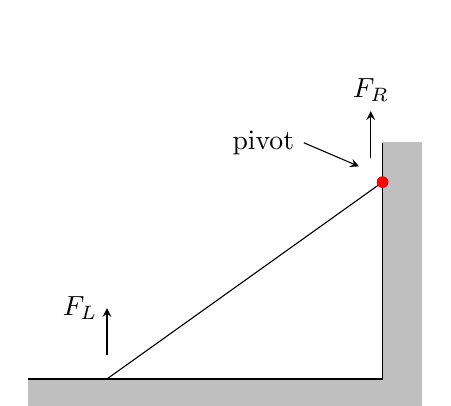
\begin{tikzpicture}
            \draw[fill,lightgray] (0,0) rectangle (5,-.5);
            \draw[fill,lightgray] (4.5,0) rectangle (5,3);
            \draw (0,0) -- (4.5,0) -- (4.5,3);
            \draw (1,0) -- (4.5,2.5) node
                [circle,fill,red,inner sep=1.5pt] (pivot) {};
            \draw[stealth-] (pivot) +(-.3,.2) -- +(-1,.5) node[left] {pivot};
            \draw[-stealth] (pivot)+(-.15,.3) -- +(-.15,.9) node[above] {$F_R$};
            \draw[-stealth] (1,.3) -- (1,.9) node[left] {$F_L$};
        \end{tikzpicture}
        \caption{A Special Stick}
        \label{pivoted plane}
    \end{figure}

    \begin{solution}
        Clearly, the rod does not experience any angular acceleration (the rod is in static equilibrium), so the net torque on the rod about the center of mass must be 0. The forces acting on the rod are the vertical forces $F_L$ and $F_R$, and gravity. Since gravity acts on the center of mass, it exerts no torque. Letting the length of the rod be l and the angle from the horizontal that the rod makes be $\theta$, the magnitude of the net torque is then:
        $$\tau = \frac{l}{2}F_R\cos \theta - \frac{l}{2}F_L\cos \theta = 0$$
        $$F_R = F_L$$
        Balancing forces in the vertical direction, we get $F_R + F_L = mg$
        Therefore, $F_R = F_L = mg/2$, or \boxed{C}
    \end{solution}
\end{pproblem}


\subsection*{Free Response Questions}
\setcounter{pproblem}{0}

\pts{10}
\begin{pproblem}
    A circular disc is cut in half, to make a semicircle of mass $m$ and radius $R$.
    \begin{enumerate}[\Alph*)]
        \item Find the moment of inertia of the new semicircle about
        the center of the original disk via integration.
        \item The semicircle is then angled at a slight angle $\theta_0\ll 1$ along its cut axis,
        and begins to oscillate with a period $T$. Find the distance from the axis of
        rotation to the center of mass of the semicircle in terms of $T$, $m$, $R$, and any fundamental constants. The moment of inertia
        of the semicircle about this axis is $mr^2/8$.
    \end{enumerate}
    \begin{minipage}{.5\textwidth}
        \begin{figure}[H]
            \centering
            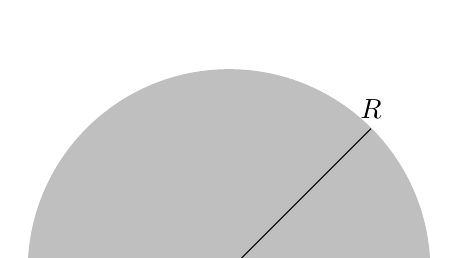
\begin{tikzpicture}[scale=1.7]
                \draw[fill,lightgray] (-1.5,0) -- (1.5,0) arc(0:180:1.5) -- cycle;
                \draw (0,0) -- (1.06,1.06) node[above]{$R$};
            \end{tikzpicture}
            \caption{Part A}
        \end{figure}
    \end{minipage}
    \begin{minipage}{.5\textwidth}
        \begin{figure}[H]
            \centering
            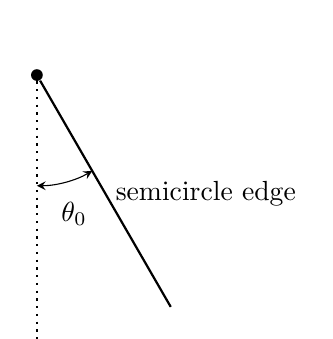
\begin{tikzpicture}[scale=1.7]
                \node[circle,fill,inner sep=1.5pt] (axis) at (0,0) {};
                \draw[thick,dotted] (axis) -- +(0,-2) node (y) {};
                \draw[thick] (axis) -- +(300:2) node (circ){}
                    node[midway, right] {semicircle edge};
                \pic [draw, stealth-stealth, "$\theta_0$", angle eccentricity=1.3,angle radius=40]
                    {angle = y--axis--circ};
            \end{tikzpicture}
            \caption{Part B, side view}
        \end{figure}
    \end{minipage}
\end{pproblem}
\begin{solution}
    \begin{enumerate}[\Alph*)]
        \item We can add up the moment of inertia for each semicircular
            ring, from $r=0$ to $r=R$. The area of each semicircular
            ring is $\text dA=\pi r\text dr$. Letting the density
            $\sigma=\dfrac{m}{\pi R^2/2}$, we then have \[
                \mathrm{d}m=\sigma\mathrm{d}A=\sigma\pi r\mathrm{d}r.
            \]
            The moment of inertia is just $\int r^2\mathrm{d}m$,
            so we have
            \begin{align*}
                I&=\int_0^Rr^2(\sigma\pi r)\mathrm{d}r\\
                &=\sigma\pi\int_0^R r^3\mathrm{d}r\\
                &=\dfrac{\sigma\pi R^4}{4} = \dfrac{mR^2}{8}
            \end{align*}

        \item Let the distance to the center of mass be $d$. Gravity
            exerts a torque of $-mgd\sin\theta$. For $\theta_0\ll1$,
            $\sin\theta\approx\theta$ so \[
                \tau_\mathrm{net}=-mgd\theta
            \]
            This is equal to $I\ddot{\theta}$, by $\tau=I\alpha$.
            Let $\omega^2=\dfrac{mgd}{I}$: in this case,
            we then have \[
                -\omega^2\theta=\ddot{\theta}
            \]
            This is the equation of an oscillation with angular frequency
            $\omega$. Therefore, the period is $T=\dfrac{2\pi}{\omega}$.
            From there, we can solve for $d$:
            \begin{align*}
                T&=2\pi\sqrt{\dfrac{I}{mgd}}\\
                &=\pi R\sqrt{\dfrac{1}{2gd}}\\
                \implies d&=\dfrac{\pi^2R^2}{2gT^2}
            \end{align*}
    \end{enumerate}
\end{solution}

\pts{10}
\begin{pproblem}
    An initially uniform disk of radius R has a circular hole with radius R/2 cut out, as shown, where the center of the hole is a distance R/2 from the center of the disk. The mass of the remaining "disk" is M. The disk is placed in a container where it can only move in the vertical direction but can still rotate. At time $t = 0$, the disk is connected to a wheel that gives the disk an angular acceleration $\alpha$ counterclockwise. 

    The center of mass of this "disk" is given to be a distance R/6 from the center of the original disk. After some time T, the disk will start to "jump" up and lose contact the lower wheel momentarily because of the circular motion of the center of mass (it moves in a circle of radius R/6)
     
    \begin{figure}[H]
        \centering
        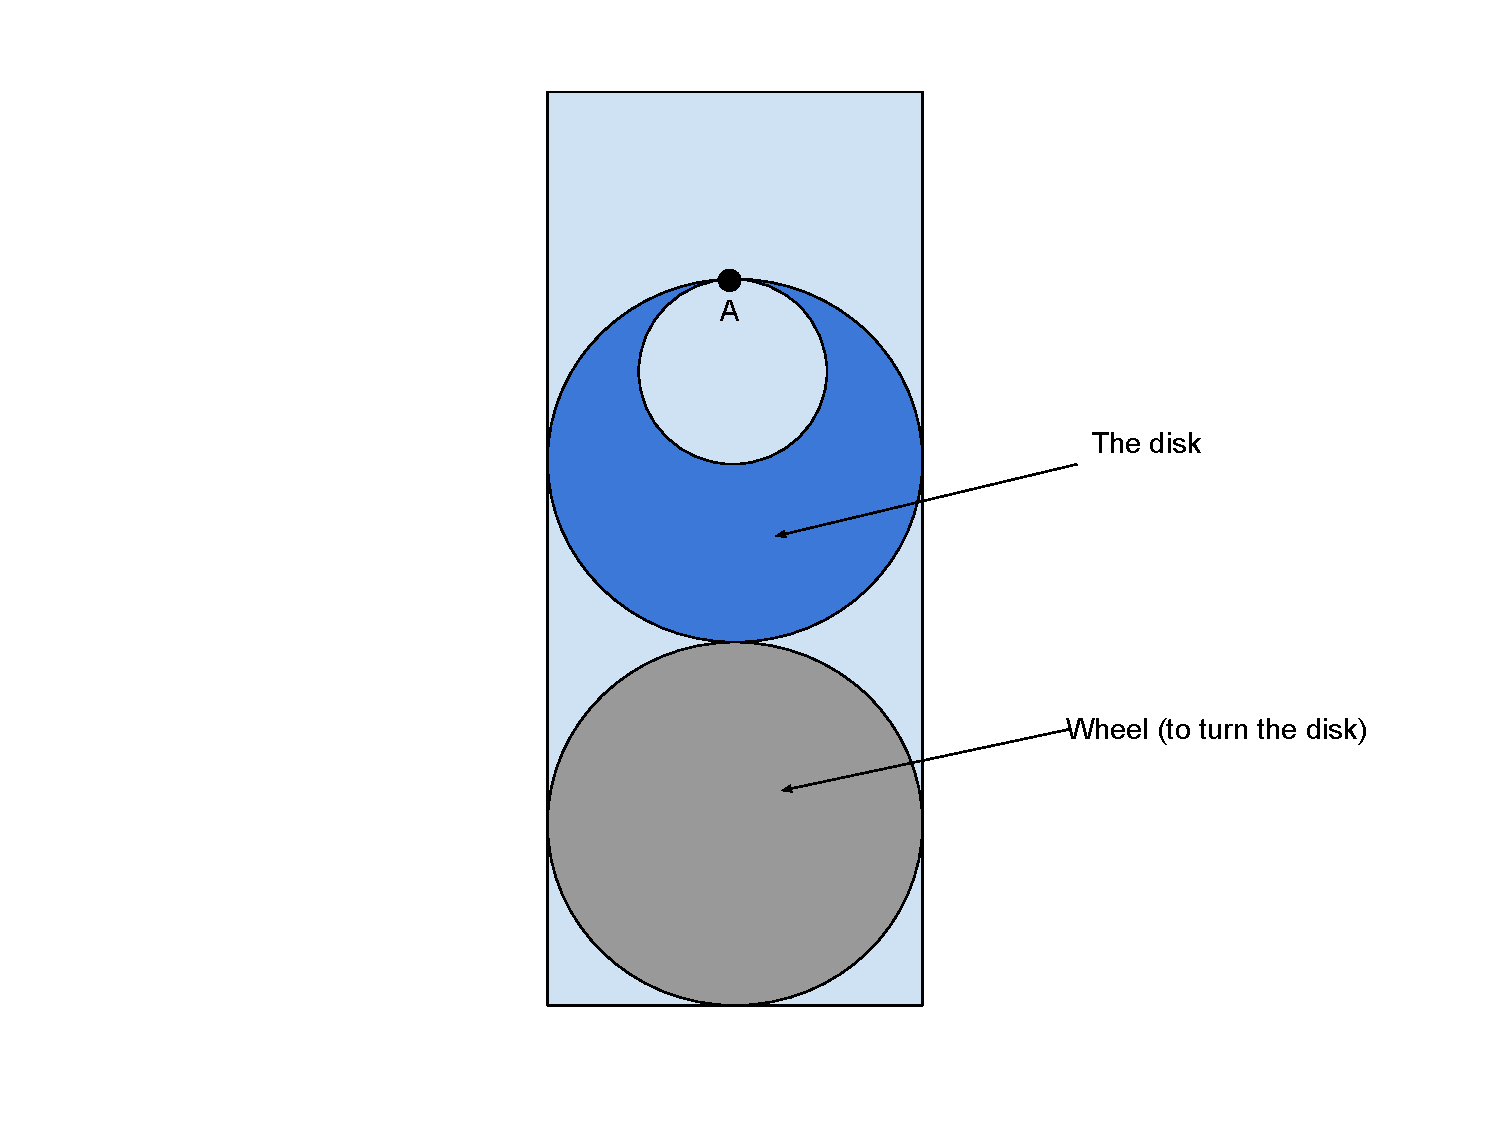
\includegraphics[scale=0.5]{rotationsTestDiskProblem (1).pdf}
    \end{figure}
    \begin{enumerate}[\Alph*)]
        \item Find the time $T$ where the disk begins to "jump" in terms of $\alpha$, $M$, $R$, and any fundamental constants. Assume that at time T, the period of the disk's rotation is much smaller than T. 
        \item At some time $t$, find the angular momentum of the disk in terms of $t$, $\alpha$, $M$, $R$, and any fundamental constants.
        \item Using your answer for part b), find the angular momentum of the disk when it first loses contact with the wheel. 
        % \item Now suppose this disk was taken out of the container and a pivot was attached to the disk at point A as shown. Provided that the disk can undergo small oscillations about this pivot point, find the period of these oscillations. 
    \end{enumerate}
\end{pproblem}
\begin{solution}
    \begin{enumerate}[\Alph*)]
        \item The disk jumps up from the wheel because the center of mass moves in a circle of radius R/6 around the center of the initial disk. Working in the rotating reference frame of the disk, there is a centrifugal force acting on the center of mass pointing radially out, which balances with the normal force from the wheel, normal forces from the side of the container, and gravity. 
        
        At the moment when the disk loses contact with the wheel, the magnitude of the normal force from the wheel on the disk is 0. Since the normal forces from the container have no vertical components, the centrifugal force must cancel with the gravitational force. The centrifugal force is maximum when the center of mass is directly above the center of the disk. At this time, the magnitude of the centrifugal force is $F_c = m\frac{R}{6}\omega ^2$. Since $F_c = F_g$
        $$m\frac{R}{6}\omega ^2 = mg$$
        $$\omega = \sqrt{\frac{6g}{R}}$$
        The time that it takes for the disk to acquire this angular velocity is $T = \frac{\omega}{\alpha} = \boxed{\frac{1}{\alpha}\sqrt{\frac{6g}{R}}}$

        Correction: this solution assumes that at time T the center of mass of the disk will be directly above the center of the disk, although this may not necessarily be true given the original wording. This question has been modified slightly for clarification. The actual answer would therefore be slightly greater than T to allow for the disk to rotate to close to that position. However, for sufficiently small values of R, the value of $\omega$ for which the disk loses contact with the wheel becomes large enough that T is a good approximation for the actual answer. 

        \item The disk rotates about its initial center, so the angular momentum is $I\omega$ where I is the moment of inertia about the center and $\omega = \alpha t$ since the angular acceleration is constant. Before the hole in the disk was made, the moment of inertia of the disk was given by $$I_0 = \frac{1}{2}m'R^2$$ where $m' = \frac{4}{3}m$ because the hole accounts for 1/4 of the area of the initial disk, so it must also account for 1/4 of the mass. Therefore,
        $$I_0 = \frac{2}{3}MR^2$$

        Now we focus on finding the moment of inertia about the center of the portion of the disk that was removed. Using the same formula for moment of inertia at the center of the disk, $I_{\text{cm, removed}} = \frac{1}{2}\frac{M}{3}(\frac{R}{2})^2 = \frac{1}{24}MR^2$. We then use the parallel axis theorem to find the moment of inertia of this section about the center of the large disk.  

        $$I_{\text{removed}} = I_{\text{cm, removed}} + \frac{M}{3}(\frac{R}{2})^2 = \frac{1}{8}MR^2$$

        The moment of inertia after the hole is made is then:
        $$I = \frac{2}{3}MR^2 - \frac{1}{8}MR^2 = \frac{13}{24}MR^2$$

        Therefore, the angular momentum is $I\omega = \frac{13}{24}MR^2\omega = \boxed{\frac{13}{24}MR^2\alpha t}$

        \item Plugging in our value for T into the answer for part b),
        $$L = \frac{13}{24}MR^2\alpha \left(\frac{1}{\alpha}\sqrt{\frac{6g}{R}}\right) = \boxed{ \frac{13}{24}MR^2 \sqrt{\frac{6g}{R}}}$$
        
    \end{enumerate}
\end{solution}

\end{document}